\subsubsection{Single layer with imposed temperature b.c.}

Let us take a single layer of material characterised by
a heat capacity $C_p$, a heat conductivity $k$
and a heat production term $H$.

\begin{center}
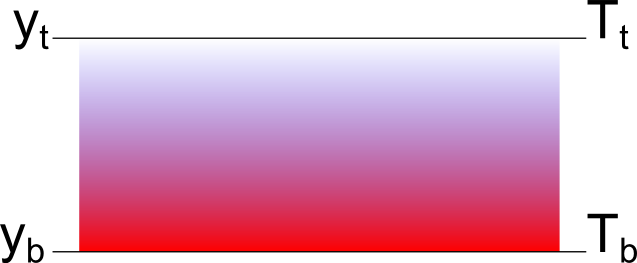
\includegraphics[width=5cm]{images/initial_temperature/tempcond.png}
\end{center}

The Heat transport equation writes
\begin{equation}
\rho C_p \left( \frac{\partial T}{\partial t} + {\vec v} \cdot {\vec \nabla} { T} \right) = 
{\vec \nabla} \cdot (k {\vec \nabla} T) + \rho H
\end{equation}
At steady state and in the absence of a velocity field, assuming
that the material properties to be independent of time and space, and 
assuming that
there is no heat production ($H=0$), this equation
simplifies to
\begin{equation}
\Delta T =0 
\end{equation}
Assuming the layer to be parallel to the $x$-axis, the temperature is
$T(x,y)=T(y)=\alpha T+ \beta$. 
In order to specify the constants $\alpha$ and $\beta$, we need two constraints.

At the bottom of the layer $y=y_b$ a temperature $T_b$ is prescribed while a temperature
$T_t$ is prescribed at the top with $y=y_t$. This ultimately yields a temperature field in
the layer given by
\begin{mdframed}[backgroundcolor=blue!5]
\[
T(y) = \frac{T_t-T_b}{y_t-y_b}(y-y_b) + T_b
\]
\end{mdframed}

If now the heat production coefficient is not zero, the differential equation
reads
\begin{equation}
 k \Delta T + H = 0 
\end{equation}
The temperature field is then expected to be of the form
\begin{equation}
T(y)= - \frac{H}{2k} y^2 + \alpha y + \beta 
\end{equation}
Supplied again with the same boundary conditions, this leads to
\[
\beta=T_b + \frac{H}{2k} y_b^2 - \alpha y_b
\]
ie,
\[
T(y) = -\frac{H}{2k} (y^2-y_b^2) + \alpha (y-y_b) + T_b
\]
and finally
\[
\alpha =  \frac{T_t-T_b}{y_t-y_b}  + \frac{H}{2k}(y_b+y_t)
\]
or,
\[
T(y) = -\frac{H}{2k} (y^2-y_b^2) + \left( \frac{T_t-T_b}{y_t-y_b}  + \frac{H}{2k}(y_b+y_t)   \right) (y-y_b) + T_b
\]

Taking $H=0$ in this equation obviously yields the temperature field obtained previously.
Taking $k=2.25$, $T_t=0C$, $T_b=550C$, $y_t=660km$, $y_b=630km$ yields the following
temperature profiles and heat fluxes when the heat production $H$ varies:
\begin{center}
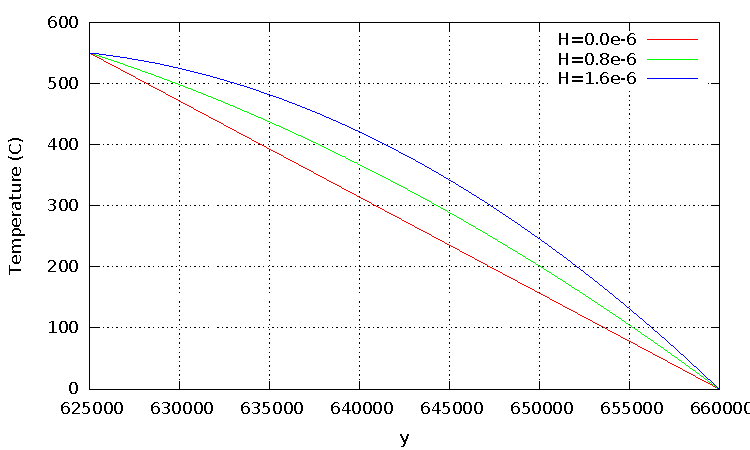
\includegraphics[width=5cm]{images/initial_temperature/temperature1.pdf}
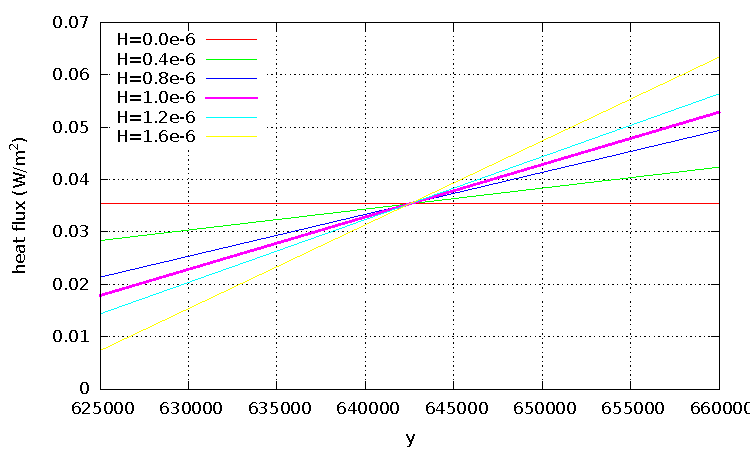
\includegraphics[width=5cm]{images/initial_temperature/heatflux1.pdf}
\end{center}
Looking at the values at the top, which are somewhat estimated to be
about $55-65mW/m^2$ \cite[table 8.6]{jama}, one sees that value $H=0.8e-6$ yields a very acceptable
heat flux.
Looking at the bottom, the heat flux is then about $0.03W/m^2$
which is somewhat problematic since the heat flux at the Moho
is reported to be somewhere between 10 and 20 $mW/m^2$ in \cite[table 7.1]{jama}.


%-----------------------------------------------------
\subsubsection{Single layer with imposed heat flux b.c.}

Let us now assume that heat fluxes are imposed at the top and bottom of the layer:
\begin{center} 
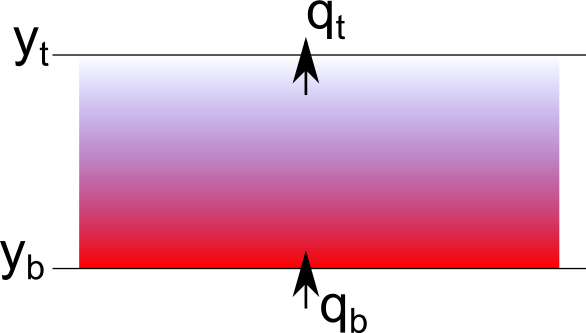
\includegraphics[width=5cm]{images/initial_temperature/tempcond2.png}
\end{center}

We start again from the ODE
\[
k \Delta T + H = 0 
\]
but only integrate it once:
\[
k \frac{dT}{dy}  + H y + \alpha  = 0 
\]
At the bottom $q=k(dT/dy)|_{y=y_b} = q_b$ and at the top
$q=k(dT/dy)|_{y=y_t} = q_t$ so that 

\todo[inline]{to finish}


 
%-----------------------------------------------------
\subsubsection{Single layer with imposed heat flux and temperature b.c. }

\begin{center}
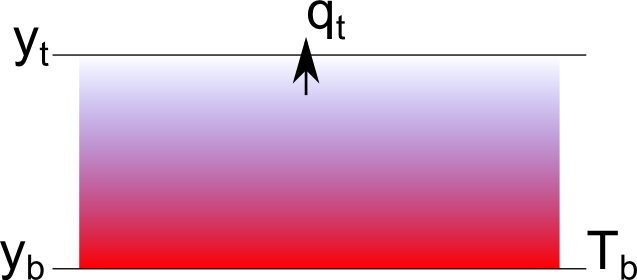
\includegraphics[width=5cm]{images/initial_temperature/tempcond3.png}
\end{center}

\todo[inline]{to finish}


%---------------------------------------------------------------
\subsubsection{Half cooling space}

TODO. 

\Literature \cite{fagm12} 

%---------------------------------------------------------------
\subsubsection{Plate model}

%.................................
\subsubsection{McKenzie slab}

When doing thermo-mechanical modelling, the initial temperature
field in the domain is of prime importance. This is 
especially true for the temperature in the slab for subduction 
modelling as its rheological behaviour is strongly temperature-dependent. 
One could easily design a simple geometrical initial field but it is 
unlikely to be close to the field of a slowly subducting slab at an angle 
in a hot mantle. 

McKenzie \cite{mcke69} derived such approximate initial field from the 
steady-state energy equation in two dimensions:
\begin{equation}
\rho C_p \vec v \cdot \vec\nabla T = k \vec\nabla^2 T
\end{equation}
We denote by $T_l$ the temperature at the base of the lithosphere
and $l$ its thickness (i.e. the thickness of the slab).

Assuming $\vec v=(v_x,0)$ yields
\[
\rho C_p v_x \frac{\partial T}{\partial x} = k \frac{\partial^2 T}{\partial x^2}
\]
and substitution of $T'=T/T_l$, $x'=x/l$ and $z'=z/l\in[0,1]$ in this equation leads to
\[
\rho C_p v_x \frac{T_l}{l}\frac{\partial T'}{\partial x'} = k \frac{T_l}{l^2}
\left( \frac{\partial^2 T'}{\partial x'^2}
+ \frac{\partial^2 T'}{\partial z'^2} \right)
\]
or 
\[
\frac{\rho C_p v_x l }{k}\frac{\partial T'}{\partial x'} = 
\frac{\partial^2 T'}{\partial x'^2}
+ \frac{\partial^2 T'}{\partial z'^2} 
\]
and finally (see Eq. 2.3 of \cite{mcke69}): 
\[
\frac{\partial^2 T'}{\partial x'^2}
- 2 R \frac{\partial T'}{\partial x'} 
+ \frac{\partial^2 T'}{\partial z'^2} =0
\]
where $R$ is the thermal Reynolds number
\[
R=\frac{\rho C_p v_x l}{2 k}
\] 
The general solution to this PDE with $T'=1$ on the top, left and right boundary is 
\[
T'(x',z')= 1 + \sum_n C_n \exp \left[ \left( R-(R^2+n^2\pi^2)^{1/2} \right) x' \right] \sin (n \pi z')
\]
We now must make an assumption about the temperature on the left boundary ($x'=0$), 
which is the temperature of the lithosphere. 
For simplicity McKenzie assumes that $T'(x'=0,z')=1-z'$ so that $C_n=2(-1)^n/n\pi$ and finally
\begin{mdframed}[backgroundcolor=blue!5]
\begin{equation}
T'(x',z')= 1 + 2\sum_n \frac{(-1)^n}{n \pi} \exp \left[ \left( R-(R^2+n^2\pi^2)^{1/2} \right) x' \right] \sin (n \pi z')
\end{equation}
\end{mdframed}

Let us build a simple temperature model for a $250\text{km}\times 50\text{km}$ slab, 
with $\rho=3000$, $C_p=1250$, $k=3$. The python code is available in {\tt images/mckenzie/mckenzie1.py}.

\begin{center}
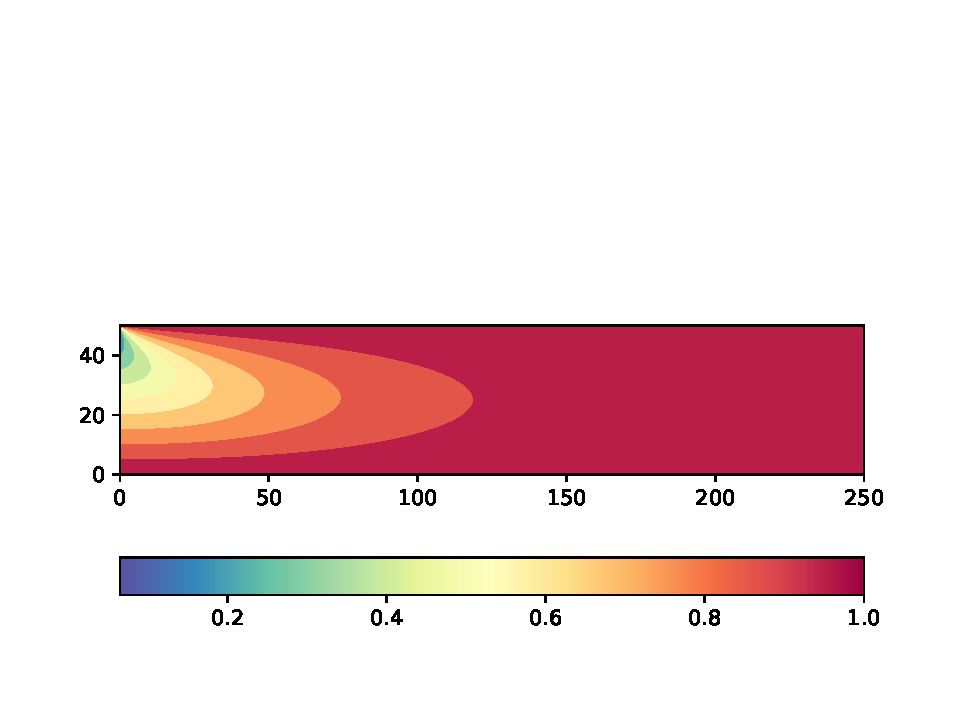
\includegraphics[width=0.32\textwidth]{images/mckenzie/temperature_vel0p5.pdf}
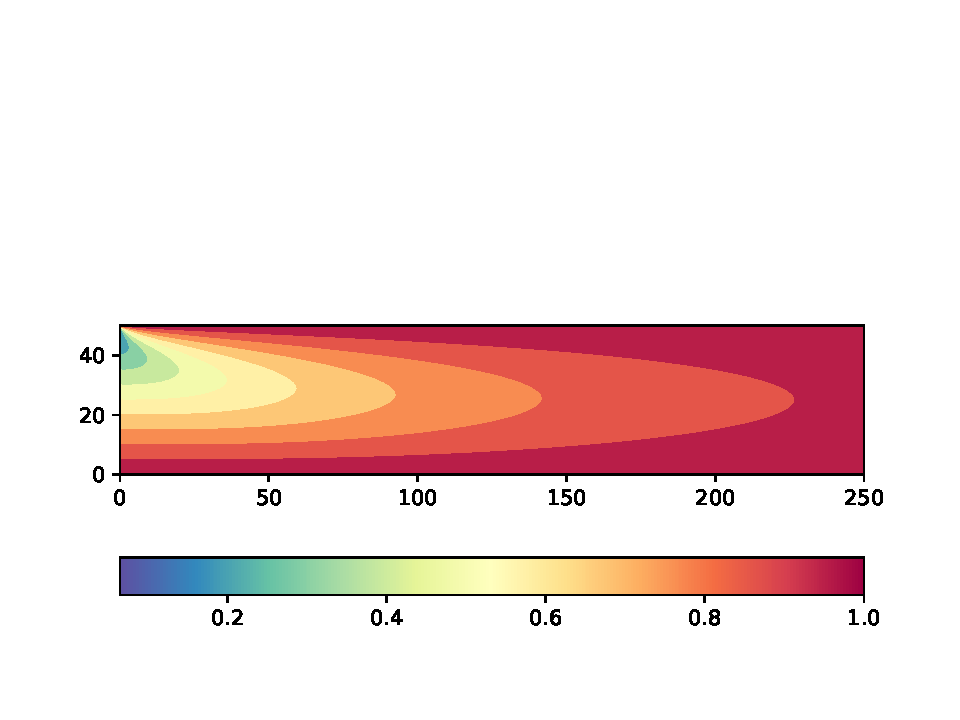
\includegraphics[width=0.32\textwidth]{images/mckenzie/temperature_vel1.pdf}
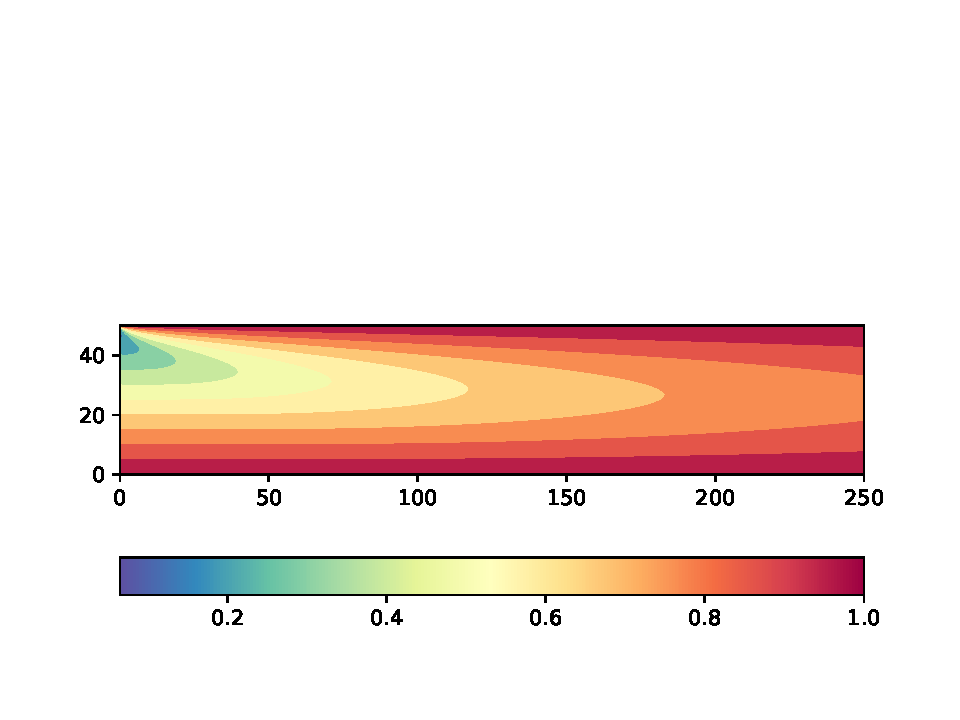
\includegraphics[width=0.32\textwidth]{images/mckenzie/temperature_vel2.pdf}\\
{\captionfont Left to right: Dimensionless temperature $T'$ in a $250\text{km}\times 50\text{km}$ slab 
for $v_x={0.5,1,2}\text{cm/year}$}
\end{center}

We logically recover the fact that the slower the slab penetrates the mantle the more 
temperature diffusion dominates over temperature advection. For $v=0.5\text{cm/year}$ we see that 
that the slab assumes a constant temperature $T'=1$ at all depthes $0\leq z' \leq 1$ for 
$x'\geq 125\text{km}$. 

Note that this field is a steady-state field, valid for a constant density, heat conductivity and 
heat capacity, zero heat production, that it implies that the velocity is constant and that the 
lithosphere temperature is linear. 

One can also embed the slab in a more realistic context, a subduction zone, involving a 
subducting lithosphere, an over-riding plate and a mantle. The domain is $1000\text{km}\times 250\text{km}$.
The mantle temperature is set to $1300\degree$. The slab dip can be varied and so can the 
velocity. The python code is available in {\tt images/mckenzie/mckenzie2.py}.

\begin{center}
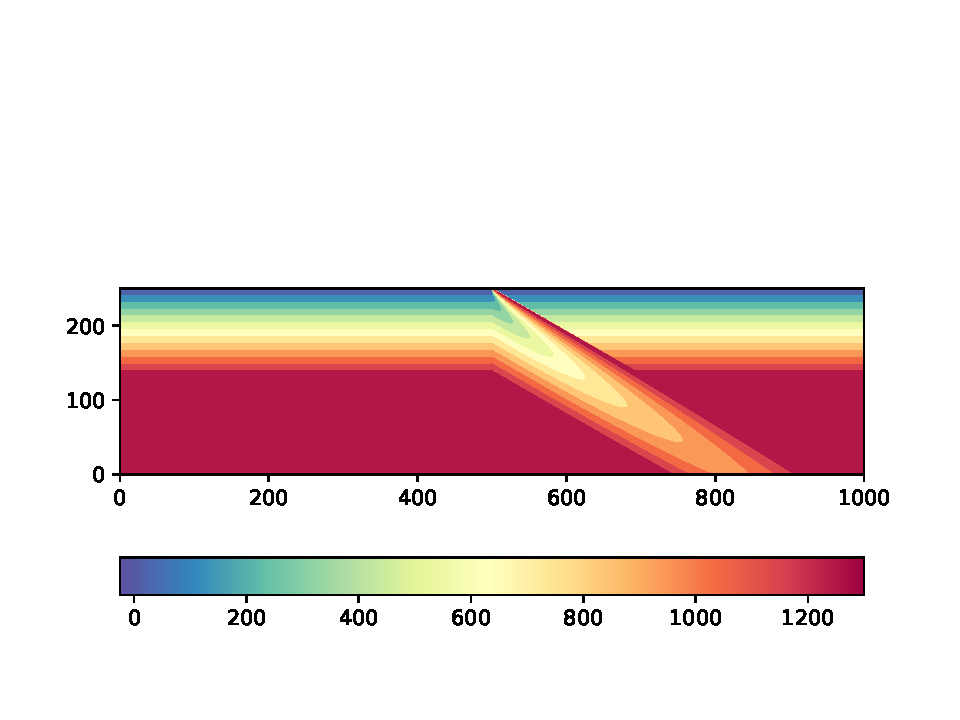
\includegraphics[width=0.32\textwidth]{images/mckenzie/temperature2_vel0p5_phi30.pdf}
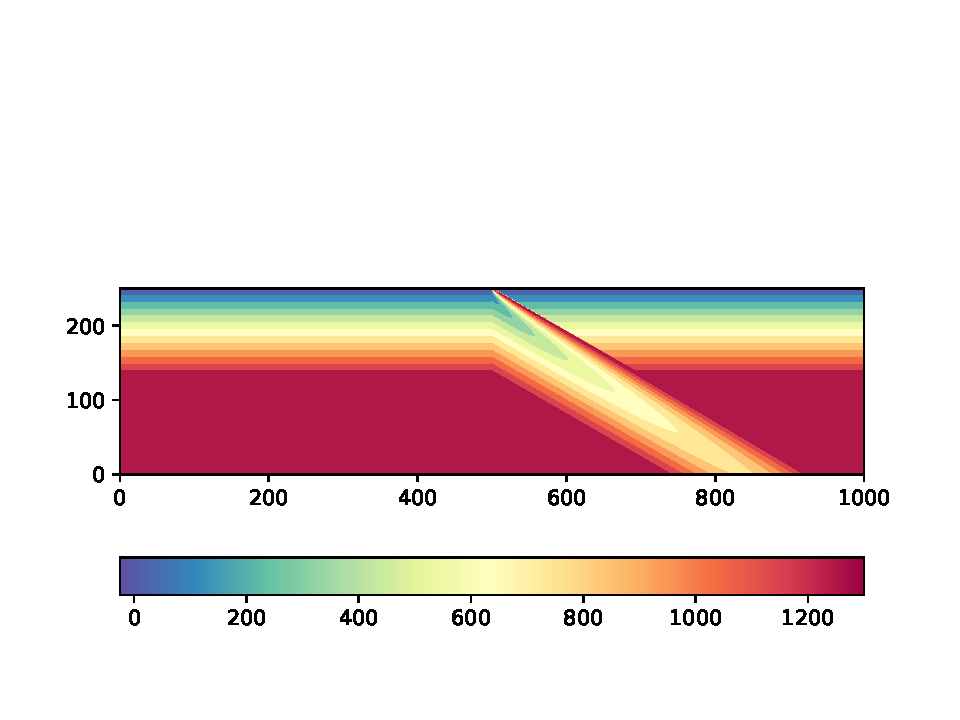
\includegraphics[width=0.32\textwidth]{images/mckenzie/temperature2_vel1_phi30.pdf}
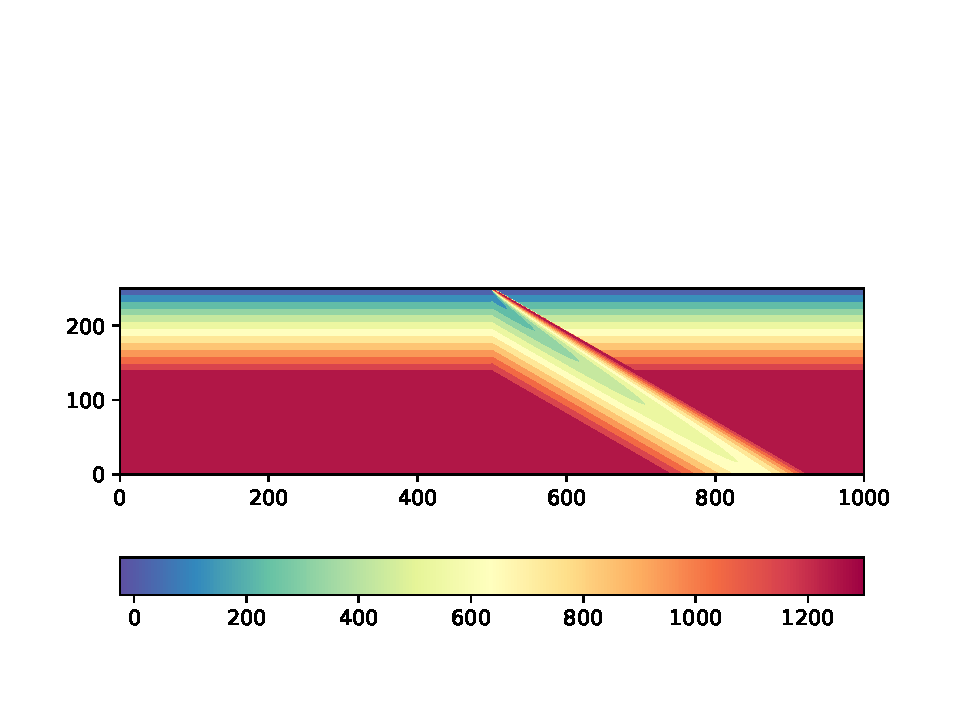
\includegraphics[width=0.32\textwidth]{images/mckenzie/temperature2_vel2_phi30.pdf}\\
{\captionfont Left to right: temperature $T$ for $v_x={0.5,1,2}\text{cm/year}$ and $\phi=30\degree$.}
\end{center}

\begin{center}
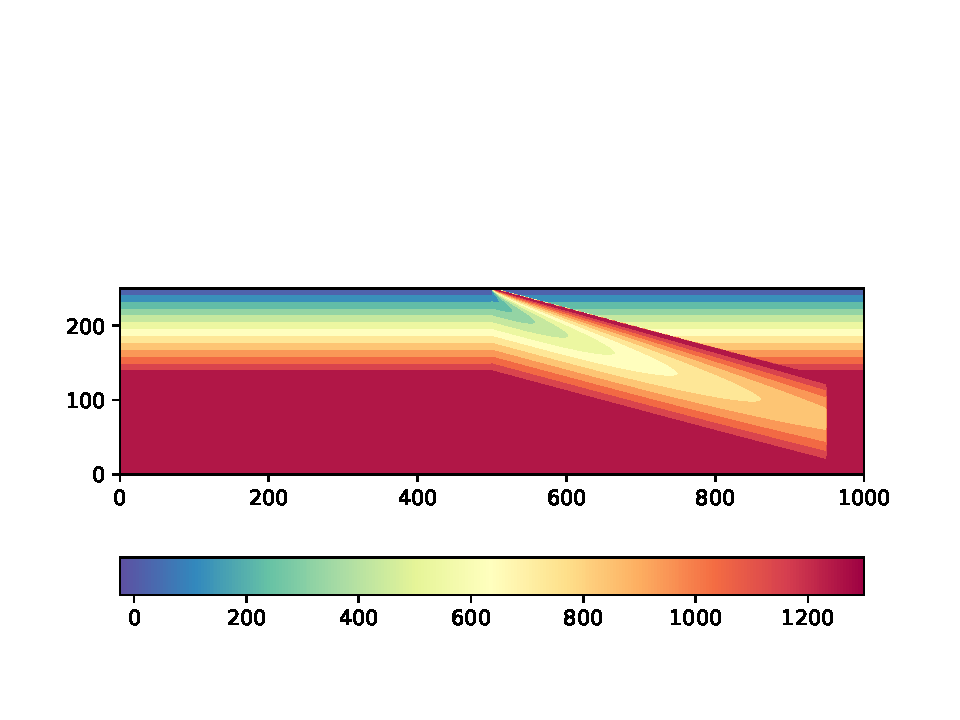
\includegraphics[width=0.32\textwidth]{images/mckenzie/temperature2_vel1_phi15.pdf}
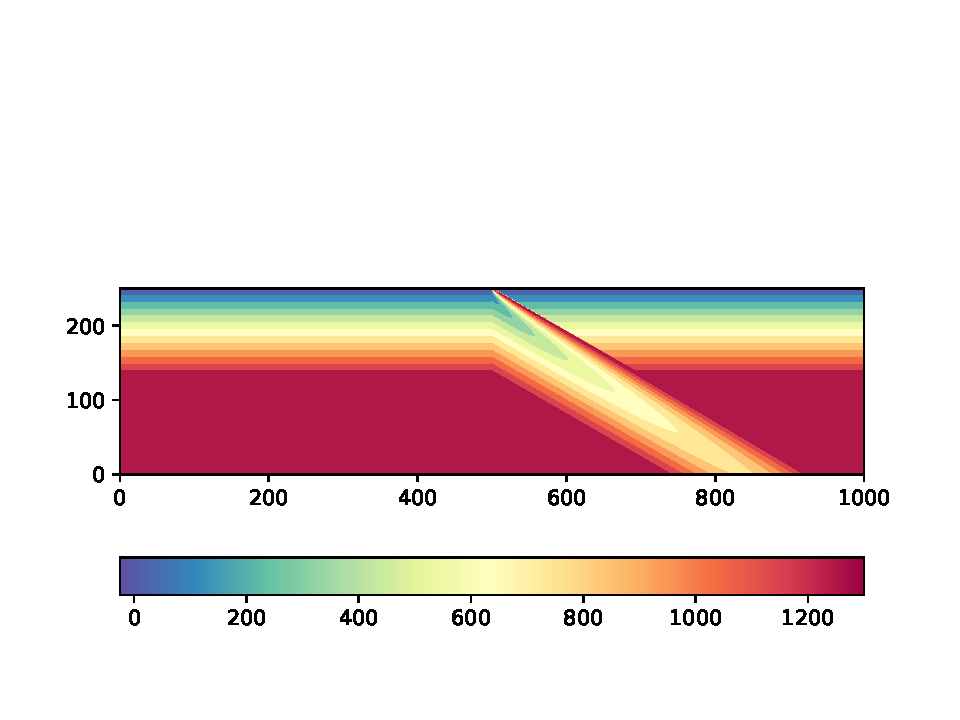
\includegraphics[width=0.32\textwidth]{images/mckenzie/temperature2_vel1_phi30.pdf}
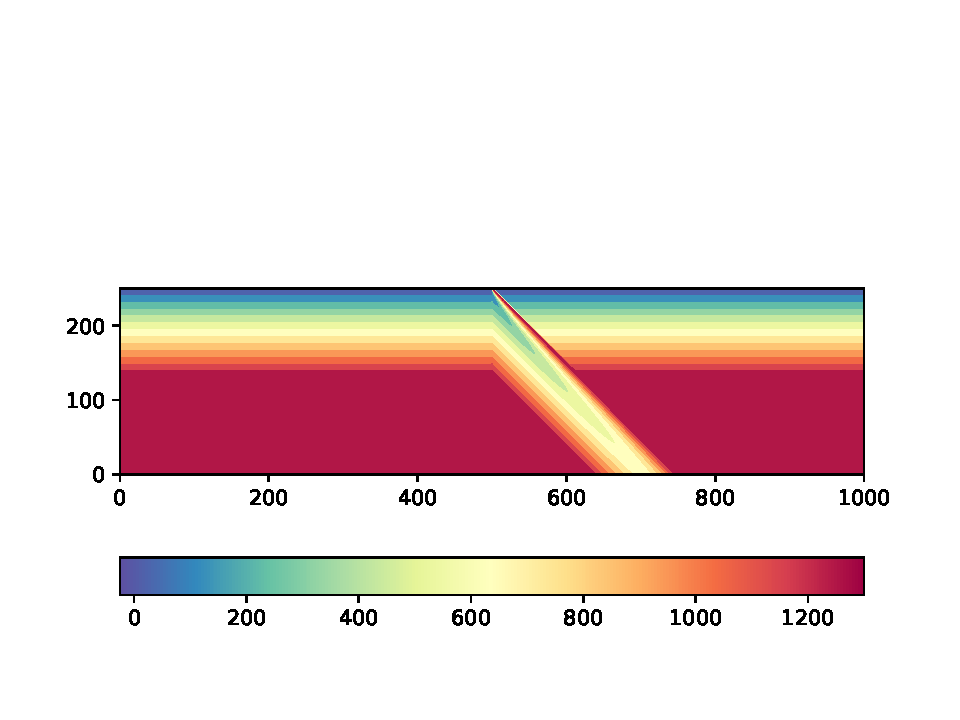
\includegraphics[width=0.32\textwidth]{images/mckenzie/temperature2_vel1_phi45.pdf}\\
{\captionfont Left to right: temperature $T$ for $v_x=1\text{cm/year}$ and $\phi={15,30,45}\degree$.}
\end{center}




%\newpage

%From \cite{mcke70}, Eq. 26:
%\[
%T(r_0) = \theta_1 \exp \left(  \frac{\alpha g}{C_p} (r_1-r_0) \right)
%\]
%where $\theta_1$ is the potential temperature of any piece of the mantle 
%at the earth's surface.
%If $x$ is measured from a depth equal to the thickness of the lithosphere down the
%dip of the slab and $z$ is measured along the normal to the slab from its lower 
%surface, then the dimensionless potential temperature in the slab is 
%\begin{eqnarray}
%\theta'(x',z')
%&=& 1+2\frac{\theta_1-273}{\theta_1} \sum_{n=1}^\infty \frac{(-1)^n}{n \pi}
%\exp \left[ \left( R-(R^2+n^2\pi^2)^{1/2} \right) x' \right] \sin n\pi z' \\
%&=& \frac{1}{\theta_1} \left\{ \theta_1+ 2 (\theta_1-273) \sum_{n=1}^\infty \frac{(-1)^n}{n \pi}
%\exp \left[ \left( R-(R^2+n^2\pi^2)^{1/2} \right) x' \right] \sin n\pi z' \right\}
%\end{eqnarray}
%where $\theta' = \theta/\theta_1$, $x'=x/l$, $z'=z/l$ and 
%with $l$ the thickness of the slab and $v$ its velocity measured down its dip.
%We denote by $\phi$ the dip of the slab so that the depth below the surface $r_1-r_0$ is given by
%$l (x' \sin \phi-z' \cos\phi)$ so that 
%\[
%T(r_0) = \theta_1 \exp \left(  \frac{\alpha g}{C_p} l (x' \sin \phi-z' \cos\phi) \right)
%\]
%The dimensionless scale height $h'$ is defined by $h'=C_p/\alpha g l$ so that
%\[
%T(r_0) = \theta_1 \exp \left[  (x' \sin \phi-z' \cos\phi)/h' \right]
%\]

%Finally,
%\[
%T(x',z')=\exp \left[  (x' \sin \phi-z' \cos\phi)/h' \right] 
%\left\{ \theta_1+ 2 (\theta_1-273) \sum_{n=1}^\infty \frac{(-1)^n}{n \pi}
%\exp \left[ \left( R-(R^2+n^2\pi^2)^{1/2} \right) x' \right] \sin n\pi z' \right\}
%\]

%\todo[inline]{BSc: create mckenzie slab temperature setup}

%......................................................................
\subsubsection{Initial temperature for global mantle convection models}

This is a difficult topic, and Gottschaldt et al \cite{gows09} list a few issues or 
facts to take into account:
\begin{itemize}
\item Frequent  impacts  may  have  determined  the  heat structure of the outer layers (Arrhenius and Lepland 2000), leading to an early thermally stable stratification. 
\item A global magma ocean (Solomatov 2000)  or  several  large  scale  melting events  (Kleine et al. 2004)  are also conceivable. 
\item Fractional crystallisation and subsequent overturn has the potential to result in compositionally or thermally   stable   layering,   too   (Elkins-Tanton et al. 2003; Zaranek and Parmentier 2004)
\end{itemize}


